\begin{center}
    \begin{tabular}{c c c}
        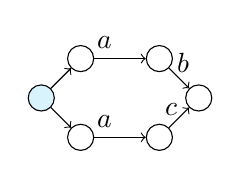
\begin{tikzpicture}
            \node[draw, circle, fill=cyan!15] (root)  at (0, 0) {};
            \node[draw, circle] (up1)   at (0.5, 0.5) {};
            \node[draw, circle] (down1) at (0.5, -0.5) {};
            \node[draw, circle] (up2)   at (1.5, 0.5) {};
            \node[draw, circle] (down2) at (1.5, -0.5) {};
            \node[draw, circle] (exit)  at (2, 0) {};

            \draw[->] (root) -- (up1);
            \draw[->] (root) -- (down1);
            \draw[->] (up1) -- node[pos=0.2, above] (a1) {$a$} (up2);
            \draw[->] (down1) -- node[pos=0.2, above] (a2) {$a$} (down2);
            \draw[->] (up2) -- node[pos=0.7, above] (b1) {$b$} (exit);
            \draw[->] (down2) -- node[pos=0.1, above] (c1) {$c$} (exit);
        \end{tikzpicture} & 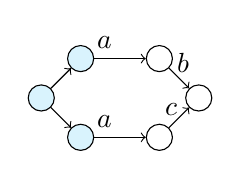
\begin{tikzpicture}
            \node[draw, circle, fill=cyan!15] (root)  at (0, 0) {};
            \node[draw, circle, fill=cyan!15] (up1)   at (0.5, 0.5) {};
            \node[draw, circle, fill=cyan!15] (down1) at (0.5, -0.5) {};
            \node[draw, circle] (up2)   at (1.5, 0.5) {};
            \node[draw, circle] (down2) at (1.5, -0.5) {};
            \node[draw, circle] (exit)  at (2, 0) {};

            \draw[->] (root) -- (up1);
            \draw[->] (root) -- (down1);
            \draw[->] (up1) -- node[pos=0.2, above] (a1) {$a$} (up2);
            \draw[->] (down1) -- node[pos=0.2, above] (a2) {$a$} (down2);
            \draw[->] (up2) -- node[pos=0.7, above] (b1) {$b$} (exit);
            \draw[->] (down2) -- node[pos=0.1, above] (c1) {$c$} (exit);
        \end{tikzpicture} & 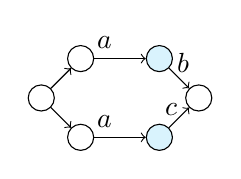
\begin{tikzpicture}
            \node[draw, circle] (root)  at (0, 0) {};
            \node[draw, circle] (up1)   at (0.5, 0.5) {};
            \node[draw, circle] (down1) at (0.5, -0.5) {};
            \node[draw, circle, fill=cyan!15] (up2)   at (1.5, 0.5) {};
            \node[draw, circle, fill=cyan!15] (down2) at (1.5, -0.5) {};
            \node[draw, circle] (exit)  at (2, 0) {};

            \draw[->] (root) -- (up1);
            \draw[->] (root) -- (down1);
            \draw[->] (up1) -- node[pos=0.2, above] (a1) {$a$} (up2);
            \draw[->] (down1) -- node[pos=0.2, above] (a2) {$a$} (down2);
            \draw[->] (up2) -- node[pos=0.7, above] (b1) {$b$} (exit);
            \draw[->] (down2) -- node[pos=0.1, above] (c1) {$c$} (exit);
        \end{tikzpicture} \\
        \textit{Initial Threads} & \textit{Free moves} & \textit{Consuming 'a'}
    \end{tabular}
    \begin{tabular}{c c}
        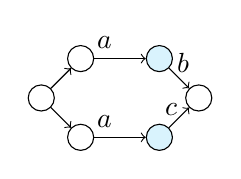
\begin{tikzpicture}
            \node[draw, circle] (root)  at (0, 0) {};
            \node[draw, circle] (up1)   at (0.5, 0.5) {};
            \node[draw, circle] (down1) at (0.5, -0.5) {};
            \node[draw, circle, fill=cyan!15] (up2)   at (1.5, 0.5) {};
            \node[draw, circle, fill=cyan!15] (down2) at (1.5, -0.5) {};
            \node[draw, circle] (exit)  at (2, 0) {};

            \draw[->] (root) -- (up1);
            \draw[->] (root) -- (down1);
            \draw[->] (up1) -- node[pos=0.2, above] (a1) {$a$} (up2);
            \draw[->] (down1) -- node[pos=0.2, above] (a2) {$a$} (down2);
            \draw[->] (up2) -- node[pos=0.7, above] (b1) {$b$} (exit);
            \draw[->] (down2) -- node[pos=0.1, above] (c1) {$c$} (exit);
        \end{tikzpicture} & 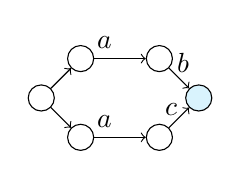
\begin{tikzpicture}
            \node[draw, circle] (root)  at (0, 0) {};
            \node[draw, circle] (up1)   at (0.5, 0.5) {};
            \node[draw, circle] (down1) at (0.5, -0.5) {};
            \node[draw, circle] (up2)   at (1.5, 0.5) {};
            \node[draw, circle] (down2) at (1.5, -0.5) {};
            \node[draw, circle, fill=cyan!15] (exit)  at (2, 0) {};

            \draw[->] (root) -- (up1);
            \draw[->] (root) -- (down1);
            \draw[->] (up1) -- node[pos=0.2, above] (a1) {$a$} (up2);
            \draw[->] (down1) -- node[pos=0.2, above] (a2) {$a$} (down2);
            \draw[->] (up2) -- node[pos=0.7, above] (b1) {$b$} (exit);
            \draw[->] (down2) -- node[pos=0.1, above] (c1) {$c$} (exit);
        \end{tikzpicture} \\
        \textit{Free moves} & \textit{Consuming 'b'}
    \end{tabular} \\ \vspace{0.3ex}
    \textit{Example of NFA simulation for the string "ab"} \\
    \textit{Cyan represents threads, and red means the edge was used during that step.}
\end{center}